\section{Stallo e multithread}
Come già menzionato, una delle funzioni principali del sistema operativo è la gestione delle risorse condivise, intese come entità passive richieste dai
thread per svolgere il proprio lavoro. Nella pratica sono per esempio il tempo di cpu, lo spazio sul disco o la memoria. In particolare, ne distinguiamo
due tipi: \begin{itemize}
    \item \textbf{Prelazionabili}: È possibile sottrarle al thread durante l'esecuzione, come la CPU o la cache.
    \item \textbf{Non prelazionabili}: Devono restare in possesso al filo, come lo spazio su disco, lucchetti mutex o eventuali periferiche.
\end{itemize}

\noindent Le risorse possono richiedere accesso esclusivo o condiviso, e in quanto tale è possibile trovare problemi di \textbf{inedia}\footnote{Chiamato
anche starvation}, ovvero quando un filo a bassa priorità attende che si liberi una risorsa costantemente in uso da altri thread la cui priorità è più
alta, ma anche di \textbf{stallo}, un'attesa circolare per le risorse dove un primo thread $A$ possiede una risorsa $r_1$ e ne attende un'altra $r_2$,
la quale è posseduta da un secondo filo $B$ che attende a sua volta $r_1$.\par
Una situazione di stallo implica anche l'inedia, ma non viceversa, perché la seconda può potenzialmente concludersi, mentre la prima necessita di un
intervento esterno per la terminazione. Inoltre, il verificarsi di uno stallo non è sempre un comportamento deterministico; per esempio, consideriamo i
due seguenti semafori che eseguono le loro primitive concorrentemente da sinistra a destra: \begin{itemize}
    \item Thread A: x.P(), y.P(), y.V(), x.V()
    \item Thread B: y.P(), x.P(), x.V(), y.V()
\end{itemize}

\noindent In quanto non deterministica, l'esecuzione delle istruzioni è soggetta a race condition, rendendo necessaria una specifica temporizzazione
mediante scheduling. In ulteriori casi è poi probabile che lo stallo capiti con risorse multiple, risultando impossibile da risolvere in modo isolato
per ogni risorsa coinvolta.\par
Supponiamo uno scenario dove un ponte può essere utilizzato per far transitare il traffico, una macchina alla volta. Ogni macchina, indipendentemente
dal lato, deve possedere il segmento di strada che deve percorrere per proseguire. Naturalmente, per attraversare il ponte, bisogna possedere il
segmento che rimarrà inaccessibile alle altre auto. In caso di stallo, una macchina dovrà indietreggiare prelazionando la sua risorsa ed è verosimile
pensare che più auto debbano indietreggiare per consentire il progresso del traffico. Inoltre, può verificarsi inedia se un lato mostra molto traffico.
Bisogna dunque conoscere che cosa causa uno stallo e come approcciarlo per risolverlo o quantomeno eluderlo.

%

\section{Caratterizzazione e gestione dello stallo}
Per prima cosa enunciamo le quattro \textbf{condizioni di Coffman}, necessarie per il verificarsi di una situazione di stallo: \begin{itemize}
    \item \textbf{Mutua esclusione}: Solo un filo alla volta può usare la risorsa.
    \item \textbf{Possesso e attesa}: Il filo che ha preso almeno una risorsa aspetta di ottenere quelle occupate da altri thread.
    \item \textbf{No prelazione}: Le risorse sono rilasciate solo volontariamente dal filo che le ha prese, quando ha finito di usarle.
    \item \textbf{Attesa circolare}: Si ha un insieme di fili in attesa dove ognuno attende che si liberi la risorsa acquisita dal processo seguente,
    fino all'ultimo che attende quella del primo.
\end{itemize}

\noindent Per visualizzare le richieste dei vari fili è possibile servirsi del \textbf{grafo di allocazione delle risorse}, che presenta un insieme di
fili $\{F_1, ..., F_n\}$ e un insieme di risorse $\{R_1, ..., R_n\}$, le quali hanno $W_i$ istanze. Ogni filo può usare una risorsa in tre modi:
richiesta(), uso() e rilascio(). In particolare, una freccia da un filo a una risorsa rappresenta una richiesta, mentre viceversa è un'assegnazione.\par
Capirlo è un buon punto di partenza, ma bisogna anche affrontare il problema dello stallo; esistono diversi approcci: \begin{itemize}
    \item \textbf{Consentire stallo e risolverlo}: Quando un sistema va in stallo si può utilizzare un algoritmo apposito per riconoscere questa
    situazione e implementare un algoritmo con il quale si forzi la prelazione delle risorse o si termini l'esecuzione di un compito.
    \item \textbf{Assicurarsi di non entrare mai in stallo}: Ciò si ottiene monitorando ogni acquisizione dei lucchetti, negando selettivamente quelli
    che possono portare a stallo.
    \item \textbf{Ignorare il problema}: Sorprendentemente è una strategia attuata da molti sistemi operativi, UNIX incluso.
\end{itemize}

\begin{figure}[h]
    \centering
    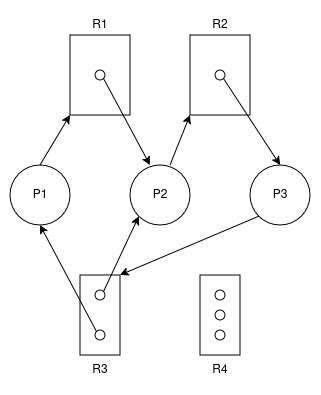
\includegraphics[width=0.4\linewidth]{Images/resourceAllocationGraph.png}
    \caption{Grafo di allocazione delle risorse}
\end{figure}

\noindent Vediamo ora un esempio di algoritmo generale per riconoscere una situazione di stallo; definiamo un $X$ vettore di $m$ interi non negativi che
rappresentano le istanze di risorse per ogni tipo. Definiamo poi i campi: \begin{itemize}
    \item $freeResources$: Risorse libere per ogni tipo.
    \item $request_x$: Richieste attuali del filo $X$.
    \item $alloc_x$: Risorse attualmente possedute dal filo $X$.
\end{itemize}

\noindent Verifichiamo se i compiti terminano automaticamente inserendoli in una struttura dati chiamata \textit{UNFINISHED}. Quelli che rimangono
salvati al suo interno saranno in stallo: \begin{lstlisting}[language=C]
    ...
    
    available = freeResources;
    // Aggiungi tutti i nodi a UNFINISHED

    do {
        done = true;
        forAll (node in UNFINISHED) {
            if (request_{node} <= available) {
                // Rimuovi il nodo da UNFINISHED
                available = available + alloc_{node};
                done = false;
            }
        }
    } while (!done);

    ...
\end{lstlisting}

\noindent Riconosciuto lo stallo, si può terminare forzatamente il filo liberando le relative risorse, ma così facendo è probabile che si lasci il
sistema in uno stato inconsistente. Alternativamente, se possibile, si possono prelazionare le risorse senza terminarlo, oppure più direttamente
riavvolgere le azioni svolte dai fili in stallo.\par
Se la soluzione che si vuole perseguire è quella di evitare lo stallo in toto, si può pensare di usare un meccanismo di \textbf{memoria virtuale}, dando
l'impressione al sistema operativo di avere risorse infinite. Se ciò non è possibile, si può direttamente evitare di condividere risorse, sebbene non
sia molto praticabile o efficiente, oppure non consentire l'attesa come si fa con le reti Ethernet in caso di collisione. Altre tecniche sono anche
quella di imporre a tutti i fili di richiedere ogni risorsa necessaria fin dall'inizio e non partire senza averle, ma è verosimile che si sovrastimi il
quantitativo, oppure di imporre a tutti i fili di richiedere le risorse in un ordine specifico per evitare usi ciclici delle risorse.\par
Un esempio di prevenzione di stallo è l'applicazione dell'\textbf{algoritmo del banchiere}, dove in un approccio ideale si dichiarano in anticipo le
risorse massime richieste e si consente a un filo di procedere se vale la relazione: \[
    \text{risorse disponibili} - \text{risorse richieste} \geq \text{risorse massime rimanenti}
\]

\noindent Un approccio meno conservativo vede un'allocazione dinamica delle risorse; si valuta ogni richiesta e la si accetta se esiste un ordinamento
di esecuzione dei fili privo di stallo. Si assume che ogni richiesta sia accettata e poi si esegue l'algoritmo di riconoscimento valutando \[
    \text{request}_{\text{node}} \leq \text{available}
\]

\noindent La richiesta sarà accettata solo se il risultato è libero da stallo. Questa strategia mantiene il sistema in uno stato \textbf{sicuro}
\footnote{Uno stato sicuro si ha quando l'esecuzione dei thread non causa situazioni di stallo.}, quindi esiste una sequenza di fili con il primo della
lista che richiede tutte le risorse a lui necessarie; quando termina la sua esecuzione, il thread seguente fa lo stesso e così via. Per esempio,
supponiamo di avere cinque processi $p_0, ..., p_4$ con quattro thread $A, B, C, D$ con il seguente stato: \begin{table}[h]
    \centering
    \begin{tabular}{|c|c|c|c|c|}
        \hline
        & assegnate & massime & richieste & disponibili\\
        \hline
        & A B C D & A B C D & A B C D & A B C D\\
        \hline
        $p_0$ & 0 0 1 2 & 0 0 1 2 & & 1 5 2 0\\
        \hline
        $p_1$ & 1 0 0 0 & 1 7 5 0 & & \\
        \hline
        $p_2$ & 1 3 5 4 & 2 3 5 6 & & \\
        \hline
        $p_3$ & 0 6 3 2 & 0 6 5 2 & & \\
        \hline
        $p_4$ & 0 0 1 4 & 0 6 5 6 & & \\
        \hline
    \end{tabular}
    \caption{Stato iniziale}
\end{table}

\noindent Per capire i valori delle risorse richieste è necessario calcolare la differenza tra le massime e le assegnate per ogni processo $p_i$. La
seconda domanda da porsi riguarda invece quali processi possono, con le attuali risorse disponibili, procedere con la propria esecuzione e terminare il
job. Valutiamo ogni caso possibile: \begin{itemize}
    \item $p_0$: Non ha ulteriori risorse richieste. Può procedere senza problemi.
    \item $p_1$: Richiede 0 7 5 0, non ci sono abbastanza risorse per i suoi fili B e C.
    \item $p_2$: Richiede 1 0 0 2, non ci sono abbastanza risorse per il suo filo D.
    \item $p_3$: Richiede 0 0 2 0, può procedere perché C ha due risorse disponibili.
    \item $p_4$: Richiede 0 6 4 2, non ci sono abbastanza risorse per i suoi fili B, C, D.
\end{itemize}

\noindent Supponiamo proceda $p_0$; alla sua terminazione verranno liberate le risorse ad esso assegnate e sommate alle disponibili, quindi diventano
1 5 3 2. La valutazione dello stato sicuro va avanti fin quando non sono terminati tutti i processi oppure se nessun processo può procedere; in tal caso
lo stato non è sicuro e si ha uno stallo. La tabella completa è la seguente, considerando che l'ordine di esecuzione dei processi è $p_0, p_2, p_3, p_4,
p_1$: \begin{table}[h]
    \centering
    \begin{tabular}{|c|c|c|c|c|}
        \hline
        & assegnate & massime & richieste & disponibili\\
        \hline
        & A B C D & A B C D & A B C D & A B C D\\
        \hline
        $p_0$ & 0 0 1 2 & 0 0 1 2 & 0 0 0 0 & 1 5 2 0\\
        \hline
        $p_1$ & 1 0 0 0 & 1 7 5 0 & 0 7 5 0 & 1 5 3 2\\
        \hline
        $p_2$ & 1 3 5 4 & 2 3 5 6 & 1 0 0 2 & 2 8 8 6\\
        \hline
        $p_3$ & 0 6 3 2 & 0 6 5 2 & 0 0 2 0 & 2 14 11 8\\
        \hline
        $p_4$ & 0 0 1 4 & 0 6 5 6 & 0 6 4 2 & 2 14 12 12\\
        \hline
        & & & & 3 14 12 12\\
        \hline
    \end{tabular}
    \caption{Valutazione completa}
\end{table}

\noindent Un'ultima cosa da notare per lo svolgimento della valutazione è come, se più processi possono avanzare, l'ordine di esecuzione non abbia
importanza per il risultato finale.